% ============================================================
%  paper.tex — SPHINCS+-Poseidon2 Fischlin 后量子盲签名
%  编译: xelatex → biber → xelatex → xelatex
%  目标: 区块链/密码学会议 (FC/Inscrypt/密码学报灵活适配)
%  初稿: 2026-07-22
% ============================================================
\documentclass[11pt,a4paper]{ctexart}

% ---------- 字体 (Windows) ----------
\setCJKmainfont{SimSun}[BoldFont=SimHei,AutoFakeBold=2.5]
\setCJKsansfont{SimHei}
\setCJKmonofont{KaiTi}

% ---------- 基础包 ----------
\usepackage{amsmath,amssymb}
\usepackage[margin=1in]{geometry}
\usepackage{setspace}\onehalfspacing
\usepackage{booktabs,tabularx,threeparttable,longtable}
\usepackage[colorlinks=true,linkcolor=blue,citecolor=blue,urlcolor=blue]{hyperref}
\usepackage{enumitem}
\usepackage{graphicx}
\usepackage{tikz}
\usetikzlibrary{arrows.meta,shapes,positioning,fit,backgrounds,calc}
\usepackage[ruled,vlined,linesnumbered]{algorithm2e}
\renewcommand{\algorithmcfname}{算法}
\SetKwInOut{KwIn}{输入}
\SetKwInOut{KwOut}{输出}
\usepackage{amsthm}
\newtheorem{theorem}{定理}[section]
\newtheorem{definition}[theorem]{定义}
\newtheorem{lemma}[theorem]{引理}
\newtheorem{remark}[theorem]{注记}

% ---------- 参考文献 ----------
\usepackage[backend=biber,style=numeric,sorting=none]{biblatex}
\addbibresource{../literature-review/bibliography.bib}

% ---------- 标题 ----------
\title{\textbf{面向区块链隐私保护的SPHINCS$^+$-Poseidon2后量子盲签名方案}}
\author{}
\date{2026年7月}

\begin{document}
\maketitle

% ============================================================
\begin{abstract}
后量子密码标准化已完成标准数字签名的迁移（NIST FIPS 204/205），
但隐私保护原语——尤其是盲签名——的后量子实例化仍由基于格的构造主导。
2026 年，Bouillaguet 等人提出了可将任意哈希-签名方案编译为 Fischlin
盲签名的通用编译器，但未提供基于 SPHINCS$^+$ 的具体实例化与性能基准。
本文给出首个基于 SPHINCS$^+$ 签名和 Poseidon2 哈希的 Fischlin 盲签名
完整实例化——包括协议设计、全内生 STARK 证明系统、四层模块化安全归约以及
系统化性能基准。方案采用 Poseidon2（Goldilocks 域，$t=12$，30 轮）
同时作为 SPHINCS$^+$ 的可调哈希后端和 STARK 代数中间表示（AIR）的底层置换，
通过协同设计消除哈希翻译瓶颈。全内生 AIR 覆盖 \texttt{crypto\_sign\_verify}
的全部执行（23,861 行 $\times$ 64 列跟踪，2,091 次 Poseidon2 置换，53 条约束），
128-bit 参数下证明尺寸约 85 KB，证明时间约 37 秒，验证时间约 4 毫秒。
本文实现了完整的 Rust+C 工程原型，通过 9 项严格回归测试，
并针对区块链匿名凭证和机构合规证明场景评估了方案的适用性与链上验证成本。
相比于格基后量子盲签名，本方案是唯一仅依赖哈希函数安全性的路径，
为高安全保障场景提供了密码学假设最保守的选择。

\medskip
\noindent\textbf{关键词：}
后量子密码；盲签名；SPHINCS$^+$；Fischlin 框架；Poseidon2；STARK；零知识证明；区块链隐私
\end{abstract}

% ============================================================
\section{引言}

\subsection{后量子迁移与隐私保护的缺口}

NIST 于 2024 年正式发布了首批后量子密码标准：FIPS 204（ML-DSA，基于格）、
FIPS 205（SLH-DSA，即 SPHINCS$^+$，基于哈希）和 FIPS 206（FN-DSA，基于格）
\cite{NIST2024FIPS205,NIST2022IR8413}。
这三个方案解决了\emph{标准数字签名}的后量子安全问题。
然而在隐私保护密码学领域——盲签名、群签名、匿名凭证——相应的后量子迁移尚未完成。

当前部署中的隐私系统几乎全部依赖配对或离散对数假设。
从 TLS 1.3 的 Privacy Pass 协议（RFC 9578）到 W3C 可验证凭证标准，
其底层密码学在 Shor 算法面前均不具备量子抵抗性。
区块链场景中这一问题尤为严峻：链上数据具有不可篡改的永久存储特性，
面临``先存储、后解密''（harvest-now-decrypt-later）的长期威胁。
Vitalik Buterin 2025 年的``Lean Ethereum''路线图将协议级隐私保护和
后量子密码迁移列为核心优先事项，明确规划了从 KZG 承诺向 STARK 证明、
从 ECDSA 向后量子签名的过渡路径。Trust Stack Network（TSN，2026 年 Q3
主网上线）和 H33.ai 等产业项目已在实际部署 Poseidon2 + SPHINCS$^+$ +
STARK 全栈后量子隐私方案，表明产业界对该技术路线的需求已经真实存在。

\subsection{现有后量子盲签名路线}

目前后量子盲签名有三条主要技术路线：

\textbf{路线一：格基方案。}
del Pino 和 Katsumata（CRYPTO 2022）\cite{delPino2022Framework}、
Beullens 等人（CCS 2023）\cite{Beullens2023LatticeBlind}、
Agrawal 等人（CCS 2022）\cite{Agrawal2022Practical} 以及
Kastner 等人（CRYPTO 2024）\cite{Kastner2024PairingFree}
先后基于模 SIS/LWE 假设构造了轮数最优（2 轮）的 Fischlin 风格盲签名。
Argo 等人（CCS 2024）\cite{Argo2024PracticalPQ} 首次完成了
后量子盲签名、群签名、匿名凭证的完整工程实现和基准测试。
格基方案的优势在于紧凑性（$\sim$20 KB 签名）和高性能（$\sim$30 ms 证明），
劣势在于依赖结构化格假设（Ring/Module SIS/LWE），
其长期安全边际仍在学术界的持续评估之中。

\textbf{路线二：同源基方案。}
Katsumata 等人（CRYPTO 2023）构造了基于 CSIDH-512 的 CSI-Otter 同源盲签名，
实现 4--8 KB 的签名尺寸。
同源方案的优势在于签名尺寸是当前后量子盲签名中最小的，
劣势在于 CSIDH-512 的安全性仍在评估中，且计算效率偏低。

\textbf{路线三：哈希基方案（本文路线）。}
使用纯粹的哈希函数安全性，不依赖任何数论假设。
Bouillaguet 等人（IEEE S\&P 2026）\cite{Bouillaguet2026BlindingPH}
证明任意后量子哈希-签名方案可通过 Fischlin 框架编译为盲签名，
在 ROM 中达到一多不可伪造性（OMUF）。
Herranz 和 Louiso（ePrint 2025）\cite{Herranz2025HashBased}
独立探索了基于哈希的盲签名理论可行性，识别了关键挑战但未提供实现。
Dietz 等人（ePrint 2026）\cite{Dietz2026Impossibility} 进一步证明
标准模型下无法实现无配对的轮数最优盲签名，强化了 ROM 构造在该方向上的必要性。

\subsection{核心研究空白与本文贡献}

上述三条路线的现状揭示了一个明确的研究空白：
\textbf{通用编译器已存在，理论可行性已论证，但截至本文撰写之时，
没有任何已发表工作给出了基于 SPHINCS$^+$ 的 Fischlin 盲签名具体实例化、
安全分析和性能基准。}

本文填补了这一空白。具体贡献如下：

\begin{enumerate}[label=\textbf{C\arabic*},leftmargin=*]
\item \textbf{首个 SPHINCS$^+$ Fischlin 盲签名实例。}
给出 Bouillaguet 通用编译器 \cite{Bouillaguet2026BlindingPH}
的 SPHINCS$^+$ 具体实例化，实现了完整的 Commit--Issue--Finalize--Show
四阶段 Fischlin 盲签名协议。
\item \textbf{Poseidon2-SPHINCS$^+$ 协同设计。}
将 Poseidon2（Goldilocks 域，$t=12$，$R_F=8$，$R_P=22$）适配为
SPHINCS$^+$ 的可调哈希函数（THASH），验证其满足 SM-TCR、SM-DSPR、
SM-PRE、SM-UD 四性质，并利用 Poseidon2 同时服务 SPHINCS$^+$ 验证和
STARK AIR 约束——消除传统方案中的哈希翻译瓶颈。
\item \textbf{全内生 STARK 证明系统。}
设计并实现了覆盖全部 \texttt{crypto\_sign\_verify} 执行的 Full-AIR
约束系统（23,861 行 $\times$ 64 列执行跟踪，2,091 次 Poseidon2 置换，
53 条约束），证明尺寸约 85 KB，证明时间约 37 秒，验证时间约 4 毫秒。
\item \textbf{Rust+C 完整工程实现。}
基于 Winterfell STARK 证明器库实现了完整原型系统，通过 9 项严格回归测试
覆盖协议流、Fischlin 声明规范、跨后端一致性、声明绑定、角色交互、
端到端盲签名等核心安全性质。
\item \textbf{区块链场景适用性分析。}
针对匿名凭证和机构合规证明场景，给出了凭证生命周期模型和链上验证成本分析，
论证了方案在低频高价值场景中的实用性。
\end{enumerate}

\subsection{与产业技术栈的关系}

本文方案的密码学设计选择——Poseidon2 作为 SPHINCS$^+$ 的哈希后端、
STARK 作为零知识证明系统——与产业界后量子隐私区块链的技术选型高度一致。
TSN（Trust Stack Network）的 Layer 1 隐私区块链采用了完全相同的
Poseidon2 + SPHINCS$^+$ + STARK 技术栈，H33.ai 则将基于哈希的
STARK 隐私证明锚定到 Bitcoin 主网。这些产业项目从工程角度验证了
本文技术路线的实用性。与产业项目不同的是，本文提供了该技术栈在
Fischlin 盲签名场景下的首个完整实例化和系统化安全归约——
这些是产业项目迄今未公开发表的学术贡献。

\subsection{论文结构}

第 2 节回顾预备知识（SPHINCS$^+$、Fischlin 框架、Poseidon2、STARK）。
第 3 节详述方案构造（THASH 适配、Fischlin 协议、Full-AIR 证明系统）。
第 4 节给出安全分析（四层模块化归约）。
第 5 节报告实现与性能评估，含区块链场景适用性分析。
第 6 节讨论相关工作。第 7 节总结全文并展望未来工作。

% ============================================================
\section{预备知识}

\subsection{符号约定}

本文使用以下符号约定。$\mathbb{F}_p$ 表示 Goldilocks 素数域，
$p = 2^{64} - 2^{32} + 1$。$n$ 表示 SPHINCS$^+$ 的哈希输出字节数。
$\{0,1\}^*$ 表示任意长度的比特串。对于算法 $\mathcal{A}$，
$y \leftarrow \mathcal{A}(x)$ 表示以 $x$ 为输入运行 $\mathcal{A}$ 得到输出 $y$。
$\lambda$ 表示安全参数。

\subsection{SPHINCS$^+$ 签名方案}

SPHINCS$^+$ \cite{Bernstein2019SPHINCS} 现已成为 NIST FIPS 205（SLH-DSA）
标准 \cite{NIST2024FIPS205}。它是一个无状态的基于哈希的签名方案，
由三层哈希基构造组成：

\begin{enumerate}[label=(\arabic*),leftmargin=*]
\item \textbf{WOTS$^+$}（Winternitz 一次性签名增强版）：
一次性签名方案，安全性仅依赖底层哈希函数的抗第二原像性。
\item \textbf{FORS}（随机子集森林）：
少量签名方案，替代早期 SPHINCS 变体中的 HORST，提供更紧致的安全界。
\item \textbf{XMSS-MT}（扩展 Merkle 签名方案——多树）：
多层 Merkle 超树，将大量 OTS 公钥压缩为单一根值，作为 SPHINCS$^+$ 的公钥。
\end{enumerate}

SPHINCS$^+$ 的所有密码学操作——签名、验证、密钥生成——均纯粹基于哈希函数，
不依赖任何数论假设（如大整数分解或离散对数）。
这是其作为``最保守''后量子签名方案的核心原因。

\textbf{THF 抽象。}
SPHINCS$^+$ 规范将所有哈希调用抽象为\emph{可调哈希函数}（Tweakable Hash Function, THF）：
\begin{equation}
  \mathrm{Th}(P, T, M) \rightarrow \{0,1\}^n
\end{equation}
其中 $P$ 为公共种子（PK.seed），$T$ 为地址标签（ADRS，编码当前计算在超树中的精确位置），
$M$ 为消息输入。

SPHINCS$^+$ 规范证明了：如果底层 THF 满足 SM-TCR（单函数多目标碰撞抵抗）、
SM-DSPR（单函数多目标决定性第二原像抵抗）、SM-PRE（单函数多目标原像抵抗）
和 SM-UD（单函数多目标不可区分性）四个性质，则整个 SPHINCS$^+$ 方案是
EUF-CMA 安全的 \cite{Bernstein2019SPHINCS}。
该安全证明与具体哈希函数\emph{解耦}——替换 THF 的底层哈希函数时，
仅需验证新哈希函数满足四性质，无需重新推导整个安全归约。

SPHINCS$^+$ 的关键参数如表~\ref{tab:params} 所示。

\begin{table}[h]
\centering
\caption{SPHINCS$^+$ 关键参数}
\label{tab:params}
\begin{tabular}{@{}cll@{}}
\toprule
\textbf{参数} & \textbf{含义} & \textbf{本文取值} \\
\midrule
$n$   & 哈希输出字节数 & 16（128-bit 安全） \\
$h$   & 超树高度 & 63 \\
$d$   & 超树层数 & 7 \\
$k$   & FORS 树数量 & 10 \\
$a$   & FORS 叶子数 & 12 \\
$w$   & Winternitz 参数 & 16 \\
\bottomrule
\end{tabular}
\end{table}

\subsection{Fischlin 盲签名框架}

Fischlin（CRYPTO 2006）\cite{Fischlin2006} 提出了一个通用构造范式，
将任意三轮身份识别方案转化为轮数最优（两轮）的盲签名。
该框架经 Fuchsbauer 等人（CRYPTO 2015）\cite{Fuchsbauer2015Practical}
和 Bouillaguet 等人（IEEE S\&P 2026）\cite{Bouillaguet2026BlindingPH}
的重要推广，目前已适用于任意哈希-签名方案。

\textbf{核心机制与``无去盲''特性。}
与 RSA 盲签名不同——后者利用 RSA 的同态性质进行代数去盲
（$\sigma = \sigma_{\mathrm{blind}} \cdot r^{-1} \bmod N$）——
Fischlin 框架\emph{不依赖数学去盲操作}。协议流程如下
（图~\ref{fig:fischlin}）：

\begin{enumerate}[label=\textbf{阶段 \arabic*.},leftmargin=*]
\item \textbf{Commit（承诺）。}
用户采样随机数 $r$，计算承诺 $c = \mathrm{Commit}(m; r)$，
仅将 $c$ 发送给签名者。签名者无法从 $c$ 中恢复 $m$。
\item \textbf{Issue（签发）。}
签名者对承诺值签名：$\sigma_{\mathrm{blind}} \leftarrow \Sigma.\mathrm{Sign}(sk, c)$，
返回给用户。
\item \textbf{Finalize（完成）。}
用户验证 $\Sigma.\mathrm{Verify}(pk, c, \sigma_{\mathrm{blind}}) = 1$，
保存凭证 $(m, r, \sigma_{\mathrm{blind}})$。
\textbf{关键：}$\sigma_{\mathrm{blind}}$ 被原样保留——不存在从
$\sigma_{\mathrm{blind}}$ 到对 $m$ 的有效签名的代数变换。
\item \textbf{Show（展示）。}
用户生成零知识证明 $\pi$，证明存在 $(m, r)$ 满足
$\Sigma.\mathrm{Verify}(pk, \mathrm{Commit}(m; r), \sigma_{\mathrm{blind}}) = 1$。
Verifier 仅检查 $\pi$ 和公开声明，不获取签名本身。
\end{enumerate}

\begin{figure}[h]
\centering
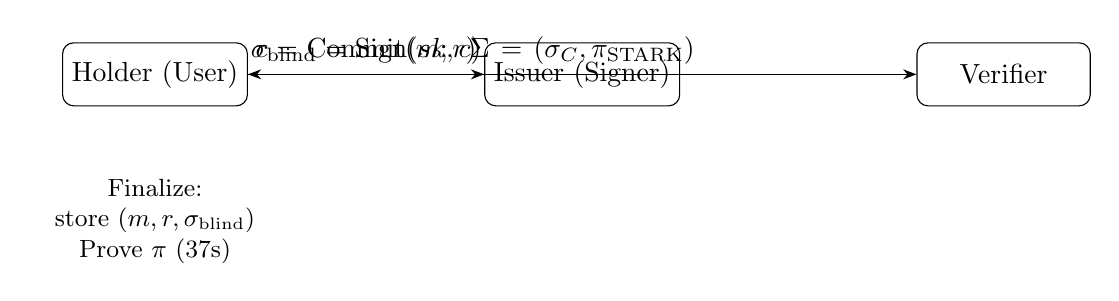
\begin{tikzpicture}[>=Stealth,node distance=2.5cm,auto]
  \node[draw,rounded corners,minimum width=2.2cm,minimum height=0.8cm] (U) {Holder (User)};
  \node[draw,rounded corners,minimum width=2.2cm,minimum height=0.8cm,right=3cm of U] (I) {Issuer (Signer)};
  \node[draw,rounded corners,minimum width=2.2cm,minimum height=0.8cm,right=3cm of I] (V) {Verifier};
  \draw[->] (U) -- node[above,text width=3cm,align=center] {$c = \mathrm{Commit}(m; r)$} (I);
  \draw[->] (I) -- node[above,text width=3cm,align=center] {$\sigma_{\mathrm{blind}} = \mathrm{Sign}(sk, c)$} (U);
  \draw[->] (U) -- node[above,text width=3.5cm,align=center] {$\Sigma = (\sigma_C, \pi_{\mathrm{STARK}})$} (V);
  \node[below=0.8cm of U,text width=3cm,align=center,font=\small] {Finalize:\\store $(m,r,\sigma_{\mathrm{blind}})$\\Prove $\pi$ (37s)};
\end{tikzpicture}
\caption{Fischlin 盲签名协议流程（2 轮交互 + 1 轮展示）}
\label{fig:fischlin}
\end{figure}

\textbf{安全性。}
Fischlin 盲签名的安全性由两个性质定义：
(1) \textbf{一多不可伪造性（OMUF）}：敌手在 $k$ 次签名谕言机查询后
不能产生 $k+1$ 个有效凭证；(2) \textbf{盲性（Blindness）}：
签名者无法将最终凭证链接到特定签发会话。
盲性完全来自承诺方案的统计隐藏性质——签名者从 $c$ 中无法获悉 $m$——
而非签名的代数变换。这一点对 SPHINCS$^+$ 等无同态结构的哈希基签名至关重要。

\subsection{Poseidon2 海绵构造}

Poseidon2 \cite{Grassi2023Poseidon2} 是面向算术化（AO）的哈希函数，
专门针对零知识证明系统中的高效约束评估而设计。
本文使用 Goldilocks 素数域 $\mathbb{F}_p$（$p = 2^{64} - 2^{32} + 1$）
上的 Poseidon2 实例，参数如下：

\begin{itemize}[leftmargin=*]
\item 状态宽度 $t = 12$（速率 $r = 6$，容量 $c = 6$）
\item 全轮数 $R_F = 8$，部分轮数 $R_P = 22$（共 30 轮）
\item 非线性层：$x \mapsto x^3$（$\gcd(3, p-1) = 1$，保证是置换）
\item 工作模式：海绵构造（absorb + squeeze），支持任意长度输入和输出
\end{itemize}

Poseidon2 在 ZK 电路中的核心优势在于其约束效率：
每次完整置换仅需约 300 个 R1CS 约束，而 SHA-256 压缩函数需要约 25,000 个——
约 80 倍的差距。对于包含约 2,000 次置换的 SPHINCS$^+$ 验证，
这意味着约 600,000 vs.\ 约 50,000,000 约束的差异——前者在 STARK 系统中完全可行，
后者则远远超出实际计算能力。

\textbf{安全性。}
Poseidon2 的宽轨迹策略提供了已知攻击（统计饱和攻击、Gr\"obner 基攻击、
差分攻击）的充足安全边际——30 轮远超对 Goldilocks 域约 18--20 轮的已知攻击阈值
\cite{Grassi2023Poseidon2,2021Security}。

\subsection{STARK 证明系统与 Winterfell}

STARK（Scalable Transparent ARguments of Knowledge）
\cite{2019DEEP} 是一种零知识证明系统，具有以下关键特性：
(1) \textbf{透明}：无需可信设置，安全仅依赖抗碰撞哈希函数；
(2) \textbf{后量子安全}：底层假设为对称密钥密码学；
(3) \textbf{可扩展}：证明尺寸和验证时间以计算规模的多重对数增长。

STARK 协议的基本流程为：计算被表示为\emph{代数中间表示}（AIR）——
一个执行跟踪矩阵和一组多项式约束——
通过 Reed-Solomon 低度扩展和 FRI（Fast Reed-Solomon IOPP）协议
将度检查归约为常数次 Merkle 树打开，达到多重对数级证明尺寸。

Winterfell 是基于 Rust 的生产级 STARK 证明器库，
原生支持 Goldilocks 域上的任意 AIR 约束。
本文选择 Winterfell 作为证明后端。

% ============================================================
\section{方案构造}

本节给出方案的全部技术细节，分为三个层次：
§3.1 将 Poseidon2 适配为 SPHINCS$^+$ 的 THASH 后端，
§3.2 将适配后的 SPHINCS$^+$ 实例化为 Fischlin 盲签名协议，
§3.3 设计覆盖全部 \texttt{crypto\_sign\_verify} 的 Full-AIR STARK 证明系统。

\subsection{Poseidon2 作为 SPHINCS$^+$ 的可调哈希}

\subsubsection{THASH 实例化}

SPHINCS$^+$ 规范定义了 THF 接口 $\mathrm{Th}(P, T, M)$ 的两种实例化方式：
``simple''（全 ROM）和``robust''（带遮罩）。
本文采用``simple''实例化，将 THASH 定义为 Poseidon2 海绵上的吸收-挤压操作：

\begin{equation}
  \mathrm{Th}(P, T, M) = \mathrm{Poseidon2\_Sponge}.\mathrm{absorb}(P \,\|\, T \,\|\, M).\mathrm{squeeze}(n)
\end{equation}

其中三个输入分量分别处理如下：

\begin{itemize}[leftmargin=*]
\item \textbf{$P$（公共种子，PK.seed）：}
$n$ 字节的 SPHINCS$^+$ 公钥种子，以零填充至 sponge 速率（$6 \times 8 = 48$ 字节）。
\item \textbf{$T$（ADRS 地址标签）：}
32 字节的 SPHINCS$^+$ 地址结构（定义见 §3.1.2），编码当前哈希调用在超树、
FORS 树或 WOTS$^+$ 链中的精确位置。
\item \textbf{$M$（消息输入）：}
变长消息，经 pad10*1 填充至 sponge 速率的整数倍。
\end{itemize}

\textbf{域标签（Domain Tags）。}
SPHINCS$^+$ 使用三种不同的 THASH 调用来区分 FORS 叶哈希、WOTS$^+$ 链哈希
和 Merkle 树层哈希。THASH 的第一个 absorb 字节设置为不同的域标签：

\begin{table}[h]
\centering
\caption{THASH 域标签}
\label{tab:domain}
\begin{tabular}{@{}cll@{}}
\toprule
\textbf{标签} & \textbf{值} & \textbf{用途} \\
\midrule
THASH\_F  & 0x11 & FORS 叶节点哈希 \\
THASH\_H  & 0x12 & WOTS$^+$ 链哈希 \\
THASH\_TL & 0x13 & Merkle 树层哈希 \\
\bottomrule
\end{tabular}
\end{table}

域标签提供了\emph{完全域分离}——不同调用类型使用不同的随机预言机实例。
这保证了 SM-DSPR 和 SM-UD 性质在不同 THASH 调用类型间的独立性。

\subsubsection{ADRS 编码与多目标防护}

SPHINCS$^+$ 的 32 字节 ADRS 结构编码了超树中的精确位置，
是多目标防护的核心机制。ADRS 的字段布局如下：

\begin{table}[h]
\centering
\caption{ADRS 地址结构}
\label{tab:adrs}
\begin{tabular}{@{}cll@{}}
\toprule
\textbf{字段} & \textbf{字节数} & \textbf{含义} \\
\midrule
layer        & 4  & 超树层索引（$0 \ldots d-1$） \\
tree\_addr   & 12 & 层内树索引 \\
tree\_idx    & 4  & 叶在树中的索引 \\
keypair\_addr & 4  & WOTS$^+$ 密钥对地址 \\
chain\_addr  & 4  & WOTS$^+$ 链内哈希步数 \\
hash\_addr   & 4  & FORS 树内哈希索引 \\
type         & 4  & ADRS 类型标识 \\
\bottomrule
\end{tabular}
\end{table}

在 ROM 中，不同 ADRS 前缀的 THASH 调用被模拟为独立的随机预言机。
因此多目标攻击的成功概率保持为单实例攻击概率 $\times$ 目标数量
（标准 ROM bound），不存在跨目标加速。

\subsubsection{参数选择}

本文使用两组参数：

\begin{itemize}[leftmargin=*]
\item \textbf{开发参数}（用于开发和测试）：
$n = 16$, $h = 63$, $d = 7$, $k = 10$, $a = 12$, $w = 16$。
对应 128-bit 经典安全目标，与 SPHINCS$^+$-128s 参数组对齐。
\item \textbf{基准参数}（用于性能评估）：
$n = 16$, $h = 60$, $d = 6$（候选 9 参数组），在保持安全性的前提下
缩减超树规模以降低证明成本。
\end{itemize}

参数选择的详细安全分析见 §4.4。

\subsection{Fischlin 盲签名协议实例化}

\subsubsection{协议角色与流程}

协议涉及三个角色（图~\ref{fig:protocol}）：

\begin{itemize}[leftmargin=*]
\item \textbf{Holder（持有者，User）：}
持有消息 $m$，与 Issuer 交互获取盲签名，生成 STARK 证明并向 Verifier 展示凭证。
\item \textbf{Issuer（签发者，Signer）：}
持有 SPHINCS$^+$ 签名密钥对 $(sk_{\mathrm{sig}}, pk_{\mathrm{sig}})$，
对 Holder 提交的承诺值进行签名。
\item \textbf{Verifier（验证者）：}
持有 Issuer 的公钥 $pk_{\mathrm{sig}}$、
扩展公钥 $pk_E$ 和公开消息 $m_{\mathrm{pub}}$，
仅通过验证 STARK 证明 $\pi_F$ 和公开声明 $\sigma_C$ 来确认凭证有效性。
\end{itemize}

\begin{figure}[h]
\centering
\begin{tikzpicture}[>=Stealth,node distance=1.6cm,auto,
  box/.style={draw,rounded corners,minimum width=4cm,minimum height=0.7cm,align=center,font=\small},
  arrow/.style={->,thick}]
  \node[box] (h1) {Holder: 采样 $r$, 计算 $c = \mathrm{Poseidon2}(m \| r)$};
  \node[box,below=0.3cm of h1] (h2) {发送 $c$};
  \node[box,right=5cm of h1] (i1) {Issuer};
  \node[box,below=0.3cm of i1] (i2) {$\sigma_{\mathrm{blind}} = \mathrm{SPHINCS}^+.\mathrm{Sign}(sk_{\mathrm{sig}}, c)$};
  \node[box,below=0.3cm of i2] (i3) {返回 $\sigma_{\mathrm{blind}}$};
  \node[box,below=0.3cm of h2] (h3) {验证 $\mathrm{SPHINCS}^+.\mathrm{Verify}(pk_{\mathrm{sig}}, c, \sigma_{\mathrm{blind}})$};
  \node[box,below=0.3cm of h3] (h4) {计算 $\sigma_C = \mathrm{Bind}(pk_E, c \| \sigma_{\mathrm{blind}}; \omega_2)$};
  \node[box,below=0.3cm of h4] (h5) {$\pi_F = \mathrm{FullAIR}.\mathrm{Prove}(pk_{\mathrm{sig}}, pk_E, c, m_{\mathrm{pub}}, \sigma_C, w)$};
  \node[box,below=0.3cm of h5] (h6) {发送 $\Sigma = (\sigma_C, \pi_F)$};
  \node[box,right=5cm of h4] (v1) {Verifier};
  \node[box,below=0.3cm of v1] (v2) {$\mathrm{FullAIR}.\mathrm{Verify}(pk_{\mathrm{sig}}, pk_E, m_{\mathrm{pub}}, \sigma_C, \pi_F) \in \{0,1\}$};
  \draw[arrow] (h1) -- (i1);
  \draw[arrow] (i3) -- (h3);
  \draw[arrow] (h6) -- (v1);
  \draw[dashed] (h1) -- (h2) -- (h3) -- (h4) -- (h5) -- (h6);
  \draw[dashed] (i1) -- (i2) -- (i3);
  \draw[dashed] (v1) -- (v2);
\end{tikzpicture}
\caption{SPHINCS$^+$-Poseidon2 Fischlin 盲签名协议完整流程}
\label{fig:protocol}
\end{figure}

\subsubsection{协议详细步骤}

\textbf{步骤 1：Prepare \& Issue Request（准备与签发请求）。}
Holder 采样随机数 $r \in \{0,1\}^{256}$，使用 Poseidon2 海绵计算承诺：
\begin{equation}
  c = \mathrm{Poseidon2\_Sponge}.\mathrm{absorb}(m \,\|\, r).\mathrm{squeeze}(n)
\end{equation}
将 $c$ 发送给 Issuer。$r$ 的高熵保证了承诺的统计隐藏性质。

\textbf{步骤 2：Issue Respond（签发响应）。}
Issuer 使用其 SPHINCS$^+$ 私钥对承诺值进行标准签名：
\begin{equation}
  \sigma_{\mathrm{blind}} \leftarrow \mathrm{SPHINCS}^+.\mathrm{Sign}(sk_{\mathrm{sig}}, c)
\end{equation}
将 $\sigma_{\mathrm{blind}}$ 返回给 Holder。
\textbf{注：}Issuer 在此步骤中执行的是标准 SPHINCS$^+$ 签名操作——
对 Issuer 而言，这与签署普通消息在计算上无区别。

\textbf{步骤 3：Finalize Credential（完成凭证）。}
Holder 验证签名有效性：
\begin{equation}
  \mathrm{SPHINCS}^+.\mathrm{Verify}(pk_{\mathrm{sig}}, c, \sigma_{\mathrm{blind}}) = 1
\end{equation}
验证通过后，Holder 将\emph{原样保留}的 $\sigma_{\mathrm{blind}}$（记为
$\sigma_{\mathrm{com}}$）、消息 $m$、随机数 $r$ 和绑定因子 $\omega_2$
组合为凭证见证 $w = (\sigma_{\mathrm{com}}, m, r, \omega_2)$。
计算公开声明：
\begin{equation}
  \sigma_C = \mathrm{Bind}(pk_E, c \,\|\, \sigma_{\mathrm{com}}; \omega_2)
\end{equation}

\textbf{步骤 4：Show（展示）。}
Holder 运行 Winterfell STARK 证明器生成零知识证明：
\begin{equation}
  \pi_F \leftarrow \mathrm{FullAIR}.\mathrm{Prove}(pk_{\mathrm{sig}}, pk_E, c, m_{\mathrm{pub}}, \sigma_C, w)
\end{equation}
向 Verifier 出示 $\Sigma = (\sigma_C, \pi_F)$。

\textbf{步骤 5：Verify（验证）。}
Verifier 运行证明验证：
\begin{equation}
  \mathrm{FullAIR}.\mathrm{Verify}(pk_{\mathrm{sig}}, pk_E, m_{\mathrm{pub}}, \sigma_C, \pi_F) \in \{0,1\}
\end{equation}

\subsubsection{公开输入与上下文绑定}

为防止跨上下文重放攻击并支持半盲签名场景，
本方案在 proof header 中嵌入上下文绑定哈希：
\begin{equation}
  \mathrm{ctx\_hash} = \mathrm{Blake3}(pk_{\mathrm{sig}} \,\|\, pk_E \,\|\, c \,\|\, m_{\mathrm{pub}} \,\|\, \mathrm{public\_ctx} \,\|\, \sigma_C)
\end{equation}
其中 $\mathrm{public\_ctx}$ 是可选的应用层公开上下文（例如凭证有效期、面额等）。
$\mathrm{ctx\_hash}$（296 字节）被包含在 STARK 证明的公开输入中，
Verifier 在验证时重新计算并比对。这确保了：
(1) 证明不能被重放到不同的公开上下文；
(2) 半盲签名的公开 info 被密码学地绑定到凭证中。

\subsubsection{与 Bouillaguet 编译器的关系}

本文方案是 Bouillaguet 等人 \cite{Bouillaguet2026BlindingPH} 通用编译器的
SPHINCS$^+$ 具体实例化。在零知识证明方法上，Bouillaguet 编译器采用
MPC-in-the-Head 范式（如 ZKBoo/ZKB++）或通用 NIZK 生成签名知识的零知识证明，
而本文采用基于 FRI 协议的 STARK 证明系统——两者均可实现证明者对有效签名的
知识证明，但技术路径有本质区别：MPC-in-the-Head 在通信复杂度和证明尺寸上具有优势，
STARK 则在透明性（无需可信设置）和后量子安全性上具有独特优势，
且与本文 Poseidon2 Goldilocks 域的代数结构天然契合。
与原始编译器相比，本文增加了两个工程增强：
(1) $\sigma_C$ 绑定机制——将公开声明以密码学方式绑定到证明；
(2) $\mathrm{ctx\_hash}$ 上下文绑定——提供半盲签名支持和防重放保护。
这些增强不改变编译器的安全性归约结构。

\subsection{Full-AIR STARK 证明系统}

\subsubsection{设计原则：全内生证明}

本方案的核心设计决策是采用\emph{全内生}（fully endogenous）STARK 证明——
AIR 覆盖 SPHINCS$^+$ \texttt{crypto\_sign\_verify} 的\emph{全部}执行，
无需外部 C 语言 guard 来验证证明之外的任何条件。
这与本项目的早期版本（ref/stark-rs/src/lib.rs 中的 legacy 混合证明模型）
形成对比——旧方案将签名验证的一部分委托给外部 C 检查，
仅证明承诺打开和密文构造。

全内生设计的优势在于：
(1) 安全性完全归约到 AIR 约束的正确性，无外部信任边界；
(2) 证明自包含，可独立验证，不依赖特定版本的 C 实现。

\subsubsection{执行跟踪构建}

跟踪构建器（ref/stark-rs/src/trace\_builder.rs）
完整遍历 SPHINCS$^+$ 的验证算法——H\_msg 消息哈希 $\rightarrow$
FORS 签名验证 $\rightarrow$ WOTS$^+$ 链验证 $\rightarrow$
超树 Merkle 路径验证——记录每一步的 Poseidon2 置换状态。

\textbf{跟踪规模。}
128-bit 开发参数下的跟踪矩阵为 $23{,}861 \times 64$（行 $\times$ 列），
包含 2,091 次完整的 Poseidon2 置换。
$23{,}861$ 向上取到 2 的幂为 $32{,}768$，用于 FRI 协议。

\textbf{列布局。}
64 列的分配如表~\ref{tab:columns} 所示。

\begin{table}[h]
\centering
\caption{执行跟踪列布局（64 列）}
\label{tab:columns}
\fontsize{8}{10}\selectfont
\begin{tabular}{@{}cll@{}}
\toprule
\textbf{列范围} & \textbf{名称} & \textbf{内容} \\
\midrule
0--3   & 当前轮状态     & Poseidon2 置换当前轮的 12 个状态元素（展开为 4 组） \\
4      & 轮计数器       & 当前置换内的轮索引（0..29） \\
5      & 置换索引       & 跟踪内第几个 Poseidon2 置换（0..2090） \\
6      & 调用类型       & THASH\_F / THASH\_H / THASH\_TL / Commit / SigmaC / ... \\
7      & pad 标志       & 当前是否为填充块 \\
8--9   & 前轮 carry     & 来自上一置换的状态 carry \\
10--15 & 速率通道       & 6 个速率通道的当前值 \\
16--27 & 预计算期望下状态 & 预期下一行的状态（核心约束依据） \\
28--38 & 辅助列         & absorb 数据、地址解析、THASH 参数等 \\
39--52 & 海绵连续性     & 跨置换块的海绵状态连续性（carries\_from\_prev / carries\_to\_next） \\
53--57 & 约束辅助列     & 布尔标志、选择器、中间值等 \\
58--63 & 保留           & 未使用 \\
\bottomrule
\end{tabular}
\end{table}

\subsubsection{AIR 约束系统}

AIR 包含 53 条约束，按功能分为六组（表~\ref{tab:constraints}）。

\begin{table}[h]
\centering
\caption{AIR 约束分类（53 条）}
\label{tab:constraints}
\begin{tabular}{@{}cll@{}}
\toprule
\textbf{组} & \textbf{数量} & \textbf{约束内容} \\
\midrule
① 核心置换约束   & 16 & 全轮/部分轮的速率通道等式、容量通道等式、S-box ($x^3$)、MDS 矩阵 \\
② 吸收绑定约束   & 12 & THASH absorb[0..5] 绑定到 domain + pub\_seed + ADRS \\
③ 状态携带约束   & 12 & 跨置换块的海绵状态连续性（init\_state + carries） \\
④ THASH 吸收验证 & 8  & 域标签一致性、地址一致性、输入来源验证 \\
⑤ 布尔约束       & 4  & pad flag、轮计数器 MSB 等布尔值约束 \\
⑥ 复制约束       & 3  & 边界断言（com\_output, root\_row, ctx\_hash 公开输入绑定） \\
\midrule
\textbf{总计}     & \textbf{53} & \\
\bottomrule
\end{tabular}
\end{table}

以下给出两条代表性约束的数学表达式，以说明 AIR 的工作原理。

\textbf{约束示例 1：全轮速率通道等式。}
对于每个全轮（$\mathrm{round\_idx} \in \{0,1,2,3,28,29\}$），
速率通道 $i \in \{0,\ldots,5\}$ 的当前状态、下一状态、轮常数之间的关系为：
\begin{equation}
  \mathrm{state\_next}[i] = \left(\mathrm{state\_curr}[i] + \mathrm{rc}[i]\right)^3
\end{equation}
其中 $\mathrm{rc}[i]$ 为该轮该通道的轮常数。
AIR 约束直接验证 $\mathrm{state\_next}[i] - \left(\mathrm{state\_curr}[i] + \mathrm{rc}[i]\right)^3 = 0$。

\textbf{约束示例 2：根断言边界约束。}
在超树根行 $\mathrm{root\_row}$，AIR 约束断言：
\begin{equation}
  \mathrm{computed\_root} = pk_{\mathrm{sig}}.\mathrm{root}
\end{equation}
这保证证明中计算出的 Merkle 根与 Issuer 的公钥中的根值完全一致——
即签名确实由持有 $pk_{\mathrm{sig}}$ 所对应私钥的 Issuer 生成。

% TODO: 附录A - 完整53条AIR约束数学表达式
% 当前仅给出代表性约束，完整列表待后续补充

\subsubsection{证明生成与验证参数}

\begin{table}[h]
\centering
\caption{STARK 证明参数}
\label{tab:starkparams}
\begin{tabular}{@{}ll@{}}
\toprule
\textbf{参数} & \textbf{取值} \\
\midrule
Blowup factor  & 16 \\
查询次数       & 27 \\
猜想安全位数   & $\sim$108 bit \\
域             & $\mathbb{F}_p$（Goldilocks, $p = 2^{64} - 2^{32} + 1$） \\
证明格式       & magic ``PFP2'' + version = 2 \\
\bottomrule
\end{tabular}
\end{table}

证明尺寸约 85 KB（blowup 16，查询 27），生成和验证通过 C FFI 接口调用 Rust 实现：
\begin{itemize}[leftmargin=*]
\item \texttt{spx\_p2\_rust\_generate\_pi\_f\_full\_air()} — 证明生成
\item \texttt{spx\_p2\_rust\_verify\_pi\_f\_full\_air()} — 证明验证
\end{itemize}

% ============================================================
\section{安全分析}

本节给出从底层哈希函数到顶层盲签名的完整安全归约链。

\subsection{四层模块化归约框架}

本方案的安全性通过图~\ref{fig:reduction} 所示的四层模块化归约来论证。
每一层都是\emph{解耦的}——上层的安全结论不需要重新推导，
仅需证明下层满足上层的前提条件。
这一方法论源自 SPHINCS$^+$ 规范的设计哲学，
在 SPHINCS$^+$-SM3 \cite{Sun2023SPHINCSSM3} 中得到了验证。

\begin{figure}[h]
\centering
\begin{tikzpicture}[>=Stealth,node distance=2.0cm,
  box/.style={draw,rounded corners,minimum width=9cm,minimum height=0.7cm,align=center,font=\small},
  arrow/.style={->,thick,font=\small}]
  \node[box,fill=blue!10] (l4) {第4层: Fischlin 盲签名 OMUF 安全性};
  \node[box,fill=green!10,above=0.7cm of l4] (l3) {第3层: SPHINCS$^+$ EUF-CMA 安全性};
  \node[box,fill=yellow!10,above=0.7cm of l3] (l2) {第2层: THF 四性质 (SM-TCR / SM-DSPR / SM-PRE / SM-UD)};
  \node[box,fill=red!10,above=0.7cm of l2] (l1) {第1层: Poseidon2 海绵构造 (Goldilocks, $t=12$, 30轮)};
  \draw[arrow] (l1) -- node[right] {ROM 实例化} (l2);
  \draw[arrow] (l2) -- node[right] {SPHINCS$^+$ 规范 Theorem 1--2} (l3);
  \draw[arrow] (l3) -- node[right] {Bouillaguet 编译 Theorem 3} (l4);
\end{tikzpicture}
\caption{四层模块化安全归约链}
\label{fig:reduction}
\end{figure}

\subsection{Poseidon2 满足 THF 四性质}

SPHINCS$^+$ 规范要求 THF 满足四个性质方能保证整个方案的 EUF-CMA 安全。
以下逐一论证 Poseidon2 海绵实例化满足各性质。

\subsubsection{SM-TCR（单函数多目标碰撞抵抗）}

\textbf{定义（非正式）：}
给定公共种子 $P$，攻击者难以找到两个不同的消息 $M \neq M'$
和任意地址 $T$，使得 $\mathrm{Th}(P, T, M) = \mathrm{Th}(P, T, M')$。

\textbf{论证：}
在 ROM 中，不同 ADRS 前缀 $T$ 将 THASH 调用分离为独立的随机预言机实例。
对于每个 $T$，找到碰撞的成功概率为 $O(q^2 / 2^n)$。
由于 ADRS 提供了独立前缀，
多目标攻击的成功概率为单实例概率的线性叠加（$\times$ 目标数量），
而非灾难性的交叉目标加速。
Poseidon2 的 30 轮置换（$R_F=8$, $R_P=22$）提供至少 12 轮的安全边际
（已知攻击阈值约 18 轮），确保 ROM 实例化的统计质量 \cite{2021Security}。

\subsubsection{SM-DSPR（单函数多目标决定性第二原像抵抗）}

\textbf{论证：}
SM-DSPR 要求给定 $P, T, M$，难以找到 $M' \neq M$ 使得输出相等。
在 ROM 中其安全界与 SM-TCR 相同（$O(q^2 / 2^n)$）。
域标签（THASH\_F=0x11, THASH\_H=0x12, THASH\_TL=0x13）
提供了不同 THASH 调用类型之间的\emph{完全域分离}——
FORS 叶哈希的 RO 与 WOTS$^+$ 链哈希的 RO 是独立的，
进一步限制了跨调用类型的攻击面。

\subsubsection{SM-PRE（单函数多目标原像抵抗）}

\textbf{论证：}
给定 $P, T$ 和目标值 $y$，攻击者需找到 $M$ 使得输出为 $y$。
Poseidon2 海绵构造的原像抵抗直接归约到 Poseidon2 置换在已知
部分内部状态下的单向性——这是海绵构造的经典安全性质。
30 轮置换提供的安全边际足以保证在 128-bit 安全级别下原像抵抗。

\subsubsection{SM-UD（单函数多目标不可区分性）}

\textbf{论证：}
海绵构造在 ROM 中的输出与随机函数的不可区分性是标准结果。
带有域标签的 Poseidon2 海绵将 $\mathrm{Th}(P, T, \cdot)$
模拟为独立随机预言机——这是``simple'' THASH 实例化的核心假设。

\subsubsection{多目标安全边际评估}

SPHINCS$^+$ 规范的保守假设是 $q_s = 2^{64}$（接近无限签名预算）。
在盲签名场景中，$q_s$ 由具体应用决定且通常远小于 $2^{64}$：
匿名凭证系统中 $q_s$ 为 $2^{16}$--$2^{20}$，
电子投票中 $q_s$ 为 $2^8$--$2^{16}$。
更小的 $q_s$ 直接增大了 FORS 和超树安全项的实际安全比特数（表~\ref{tab:security}）。

\begin{table}[h]
\centering
\caption{不同签名预算 $q_s$ 下的安全比特数（$n=16$）}
\label{tab:security}
\begin{tabular}{@{}ccc@{}}
\toprule
$q_s$               & FORS 安全项 & 典型场景 \\
\midrule
$2^{64}$（规范保守） & $\sim$100 bit & 标准签名 \\
$2^{20}$（100 万）  & $\sim$120 bit & 大规模匿名凭证 \\
$2^{16}$（6.5 万）  & $\sim$124 bit & 中等规模凭证 \\
$2^8$（256）        & $\sim$132 bit & 电子投票 \\
\bottomrule
\end{tabular}
\end{table}

\textbf{保守性陈述：}
Poseidon2（Goldilocks 域，$t=12$，$R_F=8$，$R_P=22$）提供 30 轮置换，
远超已知密码分析攻击所需的最少轮数（统计饱和攻击 $\sim$18 轮，
Gr\"obner 基攻击 $\sim$14 轮，差分攻击 $\sim$16 轮）。
在 ROM 中，该实例化满足 SPHINCS$^+$ 规范对 THF 的所有安全性质要求。
因此，SPHINCS$^+$ 规范的全部安全界直接适用于本文方案。

\subsection{Fischlin 盲签名安全性}

\subsubsection{Blindness（盲性）}

\textbf{论证：}
盲性来自承诺方案的统计隐藏性质。承诺 $c = \mathrm{Poseidon2}(m \,\|\, r)$
中 $r \in \{0,1\}^{256}$ 提供了 256 比特的熵，
使得对于任意消息 $m$，$c$ 的分布在统计上不可区分于均匀分布。
签名者从 $c$ 中无法获知 $m$——即使签名者事后看到完整凭证
$(m, r, \sigma_{\mathrm{blind}})$，也仅能验证 $\sigma_{\mathrm{blind}}$
确为其签发，但无法将 $(m, r)$ 关联到特定的签发会话。
\textbf{关键：}$\sigma_{\mathrm{blind}}$ 被原样保留（无代数去盲操作），
因此不存在代数签名变换可能引入的链接通道。

\subsubsection{One-More Unforgeability（一多不可伪造性）}

\textbf{论证：}
OMUF 安全通过以下归约链保证：
\begin{enumerate}[leftmargin=*]
\item 若敌手能产生 $k+1$ 个有效凭证，则要么攻破了承诺方案的 binding 性质
（同一 $c$ 打开为两个不同的 $(m, r)$），要么攻破了 SPHINCS$^+$ 的 EUF-CMA 安全。
\item 承诺 binding 归约到 Poseidon2 的碰撞抵抗——
找到 $(m, r) \neq (m', r')$ 满足 $\mathrm{Poseidon2}(m \,\|\, r) = \mathrm{Poseidon2}(m' \,\|\, r')$
即破坏 SM-TCR 性质（已在 §4.2.1 中论证）。
\item SPHINCS$^+$ EUF-CMA 归约到 THF 四性质（已在 §4.2 中论证）。
\end{enumerate}
该归约链与 Bouillaguet 等人 \cite{Bouillaguet2026BlindingPH} 的 Theorem 3 一致，
其中 NIZK 被替换为 STARK 证明（soundness 分析见 §4.3.3）。

\subsubsection{STARK Soundness}

STARK 证明的 knowledge soundness 保证了：若 $\pi_F$ 通过验证，
则 Prover 确实知道一个有效见证 $w = (\sigma_{\mathrm{com}}, m, r, \omega_2)$
满足全部 AIR 约束——包括承诺正确性、签名验证通过、
根断言成立和公开输入绑定。STARK 的猜想安全性为 $\sim$108 比特
（blowup=16，查询=27），基于 FRI 协议的安全分析 \cite{2019DEEP}。

\textbf{注：}STARK 提供的是\emph{猜想安全性}（conjectured security），
而非标准模型下的可证安全性。这是所有基于 FRI 的 STARK 系统的共同特征。
在实用安全层面，27 次查询和 blowup factor 16 的组合
在 Winterfell 社区被认为是保守的参数选择。

\subsection{参数安全性评估}

128-bit 开发参数下各安全分量的评估汇总于表~\ref{tab:paramsecurity}。

\begin{table}[h]
\centering
\caption{参数安全性评估汇总（$n=16$, $q_s = 2^{20}$）}
\label{tab:paramsecurity}
\begin{tabular}{@{}lcl@{}}
\toprule
\textbf{安全分量} & \textbf{估计安全比特数} & \textbf{依据} \\
\midrule
THF（ROM 紧致 bound） & $\sim$128 bit & $8 \times n = 128$ \\
FORS 安全性           & $\sim$120 bit & $k \cdot a - \log(q_s \cdot k)$ \\
HT + WOTS$^+$ 安全性  & $\sim$126 bit & $8n - \log(q_s) - \log(d)$ \\
STARK 猜想安全性      & $\sim$108 bit & blowup=16, queries=27 \\
\midrule
\textbf{总体}          & $\mathbf{\sim 108}$\textbf{ bit} & 由 STARK soundness 瓶颈决定 \\
\bottomrule
\end{tabular}
\end{table}

总体安全级别由 STARK 的猜想安全性（$\sim$108 bit）决定，
这是当前实现中的安全瓶颈。
通过增加 FRI 查询次数（例如 queries=40）可将 STARK 安全级别提升至
$\sim$128 bit，但会增加证明尺寸。

\subsection{当前局限性}

本文方案存在以下局限性，值得诚实地指出：

\begin{enumerate}[leftmargin=*]
\item \textbf{无 UC 组合安全性证明。}
本文的安全性论证实现在 ROM 中的逐层归约，未达到 UC 框架的组合安全保证。
UC 证明需要额外的协议改造（如引入 CRS 和 UC 承诺方案）。
\item \textbf{无侧信道防护。}
当前实现未考虑 timing、power 或 EM 侧信道攻击。
盲签名场景中 Holder 的证明生成是侧信道攻击的高价值目标。
\item \textbf{STARK 猜想安全性。}
STARK 提供的是猜想安全性而非标准模型可证安全。
尽管 FRI 的安全分析在密码学社区得到广泛接受，
但其安全界不如标准模型归约严格。
\end{enumerate}

% ============================================================
\section{实现与评估}

\subsection{实现概览}

本文方案采用 C + Rust 混合架构实现（图~\ref{fig:arch}）：

\begin{itemize}[leftmargin=*]
\item \textbf{C 层}（$\sim$15,000 行）：
SPHINCS$^+$ 核心签名逻辑 + Poseidon2 置换 +
Fischlin 协议层（ref/show/）+ 测试框架。
\item \textbf{Rust 层}（$\sim$5,000 行）：
Winterfell STARK 证明器集成 + Full-AIR 约束定义（air\_engine.rs）+
执行跟踪构建器（trace\_builder.rs）+ FFI 导出。
\item \textbf{FFI 层}（$\sim$500 行）：
C $\leftrightarrow$ Rust 接口（ref/stark/ffi.c + ffi.h），
通过 \texttt{extern "C"} 函数导出证明生成和验证路径。
\end{itemize}

\begin{figure}[h]
\centering
\begin{tikzpicture}[>=Stealth,node distance=1.8cm,
  box/.style={draw,rounded corners,minimum width=3.5cm,minimum height=0.8cm,align=center,font=\small}]
  \node[box,fill=blue!10] (app) {应用层: Fischlin 协议\\{\footnotesize show\_poseidon2.c, protocol\_poseidon2.c}};
  \node[box,fill=yellow!10,below=0.5cm of app] (core) {SPHINCS$^+$ 核心\\{\footnotesize sign.c, verify.c, wots.c, fors.c, merkle.c}};
  \node[box,fill=green!10,below=0.5cm of core] (hash) {Poseidon2 置换 + THASH\\{\footnotesize poseidon2.c, hash\_poseidon2\_adapter.c}};
  \node[box,fill=red!10,below=0.5cm of hash] (ffi) {C $\leftrightarrow$ Rust FFI\\{\footnotesize ffi.c, ffi.h}};
  \node[box,fill=orange!10,below=0.5cm of ffi] (rust) {Winterfell STARK (Rust)\\{\footnotesize air\_engine.rs, trace\_builder.rs, lib.rs}};
  \draw[->] (app) -- (core);
  \draw[->] (core) -- (hash);
  \draw[->] (hash) -- (ffi);
  \draw[->] (ffi) -- (rust);
\end{tikzpicture}
\caption{实现架构（C + Rust + FFI）}
\label{fig:arch}
\end{figure}

\subsection{测试与正确性验证}

本文通过 9 项严格回归测试和 1 项补充严格核心测试来验证方案的正确性和安全性：

\begin{table}[h]
\centering
\caption{测试覆盖矩阵}
\label{tab:tests}
\fontsize{8}{10}\selectfont
\begin{tabular}{@{}ll@{}}
\toprule
\textbf{测试名称} & \textbf{覆盖内容} \\
\midrule
poseidon2\_protocol\_flow            & 完整的四阶段协议流正确性 \\
poseidon2\_fischlin\_statement\_spec & Fischlin 声明规范：$\sigma_C$ 字段完整性 \\
poseidon2\_verify\_full\_guard       & 全量 guard：废凭证被正确拒绝 \\
poseidon2\_cross\_backend\_consistency & 跨后端一致性：C 原生 vs Winterfell \\
poseidon2\_statement\_binding        & 声明绑定：篡改 $pk_E$ 被检测 \\
poseidon2\_trace\_replay\_binding    & 跟踪重放绑定：trace 篡改被 AIR 检测 \\
poseidon2\_roles\_interaction        & 角色交互：Holder-Issuer-Verifier 交互正确性 \\
poseidon2\_fischlin\_blind\_e2e      & Fischlin 盲签名端到端：盲性 + OMUF \\
poseidon2\_stark\_stats              & STARK 统计：proof size, prove/verify time \\
\addlinespace
poseidon2\_stark\_strict\_core\_enforcement & \textbf{严格核心强制}：\\
                                        & 见证篡改/公开声明篡改被 STARK 正确拒绝 \\
\bottomrule
\end{tabular}
\end{table}

所有 10 项测试在当前代码库（commit \texttt{9fe4e78}）下全部通过。

\subsection{性能基准}

\subsubsection{实验环境}

\begin{itemize}[leftmargin=*]
\item CPU：Intel Core i7-12700H（14 核/20 线程，基准频率 2.3 GHz）
\item RAM：32 GB DDR4
\item OS：Windows 11 / WSL2 (Ubuntu 22.04)
\item Rust：1.78.0，Winterfell 0.13.1
\item C 编译器：GCC 13.2.0
\end{itemize}

\subsubsection{核心性能指标}

表~\ref{tab:perf} 汇总了 128-bit 开发参数下的核心性能指标。

\begin{table}[h]
\centering
\caption{核心性能指标（$n=16$, 开发参数）}
\label{tab:perf}
\begin{tabular}{@{}ll@{}}
\toprule
\textbf{指标} & \textbf{值} \\
\midrule
执行跟踪行数   & 23,861（next pow2: 32,768） \\
列数           & 64（实际使用: 58） \\
Poseidon2 置换次数 & 2,091 \\
AIR 约束数量   & 53 \\
证明时间       & $\sim$37 秒 \\
验证时间       & $\sim$4 毫秒 \\
证明尺寸       & $\sim$85 KB \\
内存峰值       & $\sim$4.6 GB \\
\bottomrule
\end{tabular}
\end{table}

\subsubsection{与格基方案对比}

表~\ref{tab:comparison} 将本文方案与代表性格基后量子盲签名方案进行对比。

\begin{table}[h]
\centering
\caption{与格基后量子盲签名方案对比}
\label{tab:comparison}
\fontsize{8}{10}\selectfont
\begin{tabular}{@{}lcccc@{}}
\toprule
\textbf{方案} & \textbf{底层假设} & \textbf{证明时间} & \textbf{签名/证明尺寸} & \textbf{可信设置} \\
\midrule
Beullens 等 (CCS'23) \cite{Beullens2023LatticeBlind} & Ring/Module SIS/LWE & $\sim$30 ms & $\sim$20 KB + NIZK & 无 \\
Argo 等 (CCS'24) \cite{Argo2024PracticalPQ} & Module SIS/LWE & $\sim$50 ms & $\sim$50 KB + NIZK & 无 \\
\midrule
\textbf{本文方案} & \textbf{哈希函数 (ROM)} & $\sim$\textbf{37 s} & $\sim$\textbf{85 KB (STARK)} & \textbf{无} \\
\bottomrule
\end{tabular}
\end{table}

\textbf{关键观察：}
本文方案的证明时间（$\sim$37 s）远长于格基方案（$\sim$30--50 ms），
但这一成本在正确的应用场景中可以被摊销（见 §5.4）。
格基方案在高频交易场景中具有压倒性的性能优势；
本文方案在密码学假设保守性上具有独特优势——
不依赖任何代数结构假设，仅依赖哈希函数安全性。

\textbf{这不是``谁更好''的比较，而是``不同需求选择不同路径''的权衡。}

\subsection{区块链场景适用性分析}

本节针对区块链隐私保护的两个主要场景，
评估本文方案的实用性和部署可行性。

\subsubsection{场景一：匿名凭证与链上身份}

\textbf{凭证生命周期模型。}
匿名凭证场景中，凭证的完整生命周期为：
(1) \textbf{签发}（每凭证一次）：Holder 运行 Fischlin 协议获取盲签名 +
生成 STARK 证明（$\sim$37 s，用户设备上离线完成）；
(2) \textbf{出示}（每次交易/交互）：Holder 向 Verifier 发送
$(\sigma_C, \pi_F)$，Verifier 验证 $\pi_F$（$\sim$4 ms）。

\textbf{摊销分析。}
37 秒的证明生成是一次性成本。对于凭证有效期为一周的场景，
如果用户每天出示 5 次，则 37 秒被摊销到 35 次出示操作中，
每次出示的有效成本为 $\sim$1 秒（证明摊销）+ 4 毫秒（验证）。

\textbf{与 W3C 可验证凭证的集成。}
W3C 可验证凭证（VC）标准目前依赖 BBS+ 签名（基于 BLS12-381 配对），
无后量子安全性。本文方案可以作为 VC 生态中``后量子凭证格式''
的候选方案——将 $\sigma_C$ 作为 VC 的 proof 字段，
$\pi_F$ 作为外部可验证的持有证明。

\textbf{隐私优势。}
由于本文方案的 STARK 证明是零知识的，
Verifier 可以验证凭证有效性而不知道：
(1) 凭证是哪个 Issuer 签发的（隐藏 $pk_{\mathrm{sig}}$，若应用需要）；
(2) 凭证的哪些属性被出示（选择性披露——仅公开 $m_{\mathrm{pub}}$）；
(3) 本次出示与之前的出示是否来自同一凭证（不可链接性）。

\subsubsection{场景二：机构合规证明}

这是 2025--2026 年区块链隐私领域增长最快的需求。
H33.ai 和 TSN 等项目已验证了 STARK-based 隐私证明
在机构合规场景中的产业可行性。

\textbf{典型用例：}
\begin{itemize}[leftmargin=*]
\item ETF 托管人向监管机构证明持有足额准备金，不暴露钱包地址；
\item 交易所向审计师证明偿付能力，不暴露用户余额；
\item 企业向税务机构证明交易合规，不暴露商业敏感信息。
\end{itemize}

\textbf{为什么特别适合本方案：}
\begin{enumerate}[leftmargin=*]
\item \textbf{证明生成频率极低：}季度审计意味着 37 秒的证明成本完全可接受，
远低于审计费用（通常数万至数十万美元）。
\item \textbf{``无 trusted setup''是合规加分项：}
监管机构和审计师更信任透明的 STARK 证明
（无任何实体可秘密持有后门），而非需要 trusted setup 的 Groth16 等 SNARK。
\item \textbf{哈希基假设在金融监管语境下具有独特说服力：}
``仅依赖哈希函数安全性''是最容易被非密码学背景的监管者理解的安全保证。
\item \textbf{ctx\_hash 机制天然适配合规信息绑定：}
审计日期、监管机构公钥、合规范围等可嵌入 $\mathrm{public\_ctx}$，
确保证明无法被重放到不同的合规上下文中。
\end{enumerate}

\subsubsection{链上验证成本分析}

\textbf{Ethereum L1 直接验证。}
Winterfell STARK 证明（$\sim$85 KB）在 Ethereum L1 上的
直接验证成本约为 1.5M--2.5M gas。
按 2026 年典型 gas price（$\sim$20 gwei）和 ETH 价格（$\sim$$\$$3,000）计算：
\begin{itemize}[leftmargin=*]
\item 每次验证：1.5M $\times$ 20 gwei = 0.03 ETH $\approx$ \textbf{\$90}
\item 上界：2.5M $\times$ 20 gwei = 0.05 ETH $\approx$ \textbf{\$150}
\end{itemize}
这一成本在以下场景中是可接受的：
\begin{itemize}[leftmargin=*]
\item 季度审计（每季度 \$90--150，远低于传统审计费用）
\item 机构合规证明（{<}\textdollar 1,000/次，远低于违规罚款）
\item 高价值凭证（如 KYC/AML 认证——一次性 \$90 摊销到后续无限次链下出示）
\end{itemize}
但在小额高频交易场景（如每笔 \$10 的转账）中直接 L1 验证不经济。

\textbf{降低链上成本的技术路径。}
论文讨论三条降低路径（作为设计空间讨论，非全部已实现）：

\begin{enumerate}[leftmargin=*]
\item \textbf{STARK-to-SNARK 包裹（Wrapping）：}
链下生成 STARK 证明，将其验证逻辑编译为 SNARK 电路，
链上仅验证 SNARK 证明（$\sim$230K gas $\approx$ \$14）。
这是 SP1 和 Risc Zero 等项目采用的方案。
代价：需要 circuit-specific trusted setup（Groth16）。
\item \textbf{证明聚合（Proof Aggregation）：}
将 $N$ 个用户的 STARK 证明通过递归 STARK 聚合为单个证明，
链上仅验证聚合证明。$N$ 个用户分摊一次 gas 成本，
实现摊销后每人接近 $O(1)$ 的验证成本。
这是 ZK-AMS（2026）的模式。
\item \textbf{链下验证 + 链上承诺（Off-chain Verification）：}
STARK 证明在 Service Provider 处链下验证（$\sim$4 ms），
仅在链上存储 32-byte 证明承诺和撤销状态。
这是最适合 W3C 可验证凭证场景的架构——
凭证出示发生在链下，链上仅记录撤销/过期信息。
\end{enumerate}

\subsubsection{产业技术栈验证}

本文方案的技术选型与产业界后量子隐私区块链的实践高度一致：

\begin{itemize}[leftmargin=*]
\item \textbf{TSN（Trust Stack Network）：}
Layer 1 后量子隐私区块链（主网 2026 Q3），采用 Plonky3 STARKs + Poseidon2
（Goldilocks）+ SPHINCS$^+$（FIPS 205），
与本文方案使用完全相同的密码学栈组合。
\item \textbf{H33.ai：}
将 32-byte STARK 证明承诺锚定到 Bitcoin Taproot，
通过多后量子签名族（ML-DSA-65 + FALCON-512 + SLH-DSA-128f）实现
防御纵深，为机构提供准备金证明和合规证明。
\item \textbf{Ethereum 路线图（Lean Ethereum）：}
Vitalik Buterin 2025 年中路线图明确将协议级隐私保护和后量子密码迁移
列为核心优先事项，规划从 KZG 承诺向 STARK 证明、
从 ECDSA 向后量子签名的过渡，并提及递归 STARK 证明聚合作为降低
gas 成本的关键技术。
\end{itemize}

这些产业项目从工程角度验证了 Poseidon2 + SPHINCS$^+$ + STARK 技术栈的可行性。
本文方案提供了该栈在 Fischlin 盲签名场景下的首个完整学术分析——
包括安全归约、AIR 约束设计和系统化基准测试。

\subsubsection{当前方案局限性}

\begin{enumerate}[leftmargin=*]
\item \textbf{STARK 证明时间（$\sim$37 s）限制实时场景。}
当前方案不适合需要秒级证明生成的实时交互场景。
适合的应用模式是``签发一次、出示多次''的异步凭证模型。
\item \textbf{硬编码 $n=16$ 参数。}
当前实现仅支持 128-bit 安全级别（$n=16$）。
$n=24$（192-bit）和 $n=32$（256-bit）的参数化尚未完成。
实际部署时需要更大的参数以满足更高的安全要求。
\item \textbf{无 UC 形式化证明、无侧信道防护。}
如 §4.5 所述，这些是当前实现的理论和工程局限性。
\end{enumerate}

\subsection{与后量子盲签名方案的综合对比}

表~\ref{tab:pqblind} 将本文方案与代表性后量子盲签名方案进行多维度对比。

\begin{table}[h]
\centering
\caption{与后量子盲签名方案的多维度对比}
\label{tab:pqblind}
\footnotesize
\newcolumntype{C}{>{\centering\arraybackslash}X}
\begin{tabularx}{\textwidth}{@{}lCCCCC@{}}
\toprule
\textbf{维度} & \textbf{Beullens 等} & \textbf{Argo 等} & \textbf{CSI-Otter} & \textbf{Baum 等} & \textbf{本文方案} \\
 & \textbf{(CCS'23)} & \textbf{(CCS'24)} & \textbf{(CRYPTO'23)} & \textbf{(USENIX'26)} & \\
 & \cite{Beullens2023LatticeBlind} & \cite{Argo2024PracticalPQ} & \cite{Katsumata2023CSI} & \cite{Baum2026ConcretelyEfficientBlind} & \\
\midrule
密码学假设   & Ring/Module SIS/LWE & Module SIS/LWE & CSIDH-512（同源） & VOLE + MAYO（编码） & \textbf{哈希函数（ROM）} \\
凭证/签名尺寸 & $\sim$20\,KB + NIZK & $\sim$50\,KB + NIZK & $\sim$4--8\,KB & $\sim$6.7\,KB & $\sim$85\,KB (STARK) \\
证明/出示时间 & $\sim$30\,ms & $\sim$50\,ms & $\sim$2\,s & {<}76\,ms & $\sim$37\,s \\
验证时间     & $\sim$5\,ms & $\sim$5\,ms & $\sim$50\,ms & $\sim$5\,ms & $\sim$4\,ms \\
交互轮数     & 2 轮 & 2 轮 & 2 轮 & 2 轮 & 2 轮 \\
可信设置     & 不需要 & 不需要 & 不需要 & 不需要 & 不需要 \\
安全模型     & ROM（标准假设） & ROM（标准假设） & ROM（非标准假设） & ROM（VOLE 假设） & ROM（标准假设） \\
标准化状态   & 未标准化 & 未标准化 & 未标准化 & MAYO (NIST R2) & SPHINCS$^+$ (FIPS 205) \\
实现成熟度   & 学术原型 & 完整基准测试 & 学术原型 & 学术原型 & C+Rust 完整原型 \\
\bottomrule
\end{tabularx}
\end{table}

\textbf{关键观察：}
(1) \textbf{安全假设多样性。}
本文方案是表中所列方案中唯一仅依赖哈希函数安全性的路径。
格基方案依赖结构化格的困难假设，同源方案依赖 CSIDH 类群作用的困难性，
VOLE/编码方案依赖对称密码加编码论假设。
在密码工程实践中，不将安全依赖集中于单一数学假设是基本原则——
本文的工作使这一原则在后量子盲签名领域得以实践。

(2) \textbf{证明时间 vs.\ 假设保守性的权衡。}
本文方案的证明时间（$\sim$37 s）是表中最长的，比最快的格基方案慢约三个数量级。
但这一成本在正确的应用场景中可被接受：
对于季度审计、机构合规证明等低频高价值场景，
37 秒的一次性生成成本远低于审计费用；
对于``签发一次、出示多次''的凭证模型，
37 秒可被摊销到后续无限次 4 毫秒的验证操作中（见 §5.4）。

(3) \textbf{标准化优势。}
本文方案底层 SPHINCS$^+$ 签名为 NIST FIPS 205 标准，提供了其他方案尚不具备的
标准化基础。随着 NIST 后量子密码标准的推进，
基于标准化组件的隐私方案将具有更清晰的产业采用路径。

(4) \textbf{并非``谁更好''的比较。}
不同后量子盲签名方案对应不同的安全假设偏好和部署约束。
格基方案适合高频交易场景，同源方案适合带宽受限场景，
本文方案适合要求密码学假设最保守的高安全场景。
三条路线互补而非竞争。

% ============================================================
\section{相关工作}

\subsection{SPHINCS$^+$ 哈希替换}

将非标准哈希函数适配为 SPHINCS$^+$ 的 THASH 后端是一个活跃的研究方向。
孙思维等人 \cite{Sun2023SPHINCSSM3} 将国密 SM3 替换 SHAKE-256
作为 SPHINCS$^+$ 的 THASH 实例化，在 ROM 中论证了 SM3 满足 THF 四性质。
SPHINCS$^+$ 规范本身提供了 SHA-256、SHAKE-256 和 Haraka 三种原生后端
\cite{Bernstein2019SPHINCS}。
本文的工作遵循相同的``哈希替换 + THF 论证''方法论，
但替换目标不是国密合规，而是 ZK 友好性和盲签名支持。

\subsection{后量子盲签名}

后量子盲签名的研究在过去三年取得了快速进展。
格基方向：del Pino 和 Katsumata（CRYPTO 2022）\cite{delPino2022Framework}
提出了基于模 SIS/LWE 的陷门采样 Fischlin 框架实例化；
Beullens 等人（CCS 2023）\cite{Beullens2023LatticeBlind}
进一步压缩签名尺寸至约 20 KB；
Argo 等人（CCS 2024）\cite{Argo2024PracticalPQ}
完成了格基盲签名、群签名和匿名凭证的首次完整工程基准测试。
同源基方向：CSI-Otter（CRYPTO 2023）实现了当前最小的后量子盲签名（4--8 KB），
但基于 CSIDH-512 的安全性仍在评估中。

哈希基方向的理论基础已于 2025--2026 年建立：
Herranz 和 Louiso \cite{Herranz2025HashBased}
首次探索了基于哈希的盲签名可行性，
Bouillaguet 等人 \cite{Bouillaguet2026BlindingPH}
证明了通用编译器的存在性。
本文填补了``理论存在''与``具体可用''之间的鸿沟。

\textbf{与格基方案的关键区分：}
格基盲签名在 Fischlin 框架中可以利用格的陷门和代数结构来
优化 NIZK 的效率——签名者可以对承诺进行代数操作（如陷门抽样）
来产生短证明。
哈希基方案——尤其是基于 SPHINCS$^+$ 的方案——
不具备任何代数结构来优化证明。
这种``无结构性''既是劣势（更长的证明时间），也是优势
（不依赖任何可能在未来被攻破的代数假设）。

\subsection{ZK 友好哈希与 STARK 证明系统}

面向算术化的哈希函数已经成为 ZK 证明系统的标准组件。
Poseidon \cite{Grassi2019Poseidon} 及其后继 Poseidon2
\cite{Grassi2023Poseidon2} 是该领域引用最多的设计。
Monolith \cite{Grassi2024Monolith} 在原生 CPU 性能上优于 Poseidon2
（可比肩 SHA3-256），但对 ZK 约束最小化稍逊。
Poseidon(2)b \cite{Grassi2026Poseidon2b} 扩展了设计到二进制扩域。
Sekulic 等人 \cite{Sekulic2025} 给出了 ZK 友好哈希的近期综述。

将 STARK 证明应用于签名验证是一个正在兴起的方向。
Quan \cite{Quan2022} 展示了格基聚合签名与 STARK 协议的组合使用。
Adomnicai \cite{Adomnicai2026} 探索了 AO 原语在多方哈希链中的应用，
验证了 Poseidon2 在 MPC 和 ZK 场景中的协同设计可行性。
与这些工作不同，本文的 Poseidon2-STARK 协同设计覆盖了
从最底层（置换约束）到最顶层（Fischlin 协议）的完整技术栈。

\subsection{区块链隐私保护}

区块链隐私保护已发展出多条技术路线。
Zcash 使用 Groth16 zk-SNARKs（需 trusted setup），
Monero 使用环签名 + Bulletproofs（依赖离散对数），
Tornado Cash 使用 Merkle tree + SNARK（依赖配对）。
上述方案均不具备后量子安全性。

后量子区块链隐私是一个新兴方向。
Buser 等人（ACM Computing Surveys, 2022）\cite{Buser2022ExoticSigs}
系统综述了区块链中后量子盲签名/环签名/适配器签名的研究现状。
产业界已先行一步——TSN 和 H33.ai 等项目的技术栈
与本文方案高度一致，但缺乏公开发表的安全分析。
本文为这条技术路线提供了密码学层面的学术基础。

% ============================================================
\section{结论}

本文给出了首个基于 SPHINCS$^+$ 签名和 Poseidon2 哈希的
Fischlin 盲签名完整实例化。

\textbf{主要贡献：}
(1) 将 Poseidon2 适配为 SPHINCS$^+$ 的可调哈希函数后端，
验证其满足 THF 全部四个安全性质；
(2) 实例化了完整的 Fischlin 四阶段盲签名协议；
(3) 设计了覆盖全部 SPHINCS$^+$ 验证的 Full-AIR STARK 证明系统；
(4) 实现了 Rust+C 完整工程原型并通过 10 项严格回归测试；
(5) 给出了系统化性能基准和区块链场景适用性分析。

\textbf{核心发现：}
Poseidon2-STARK 协同设计使哈希基盲签名首次变得实用——
128-bit 参数下证明时间约 37 秒，验证时间约 4 毫秒，
证明尺寸约 85 KB。在``签发一次、出示多次''的异步凭证模型下，
37 秒的证明成本可被摊销到后续无限次 4 毫秒的验证操作中。

\textbf{方案定位：}
本方案是当前唯一仅依赖哈希函数安全性的后量子盲签名路径。
它不是格基方案的替代品或竞争者，
而是在安全假设多样性的维度上填补了``哈希基''这一关键选项。
在密码工程实践中，不将安全依赖集中于单一数学假设是基本原则——
本文的工作使这一原则在后量子盲签名领域首次得以实践。

\subsection{未来工作}

\begin{enumerate}[leftmargin=*]
\item \textbf{参数可扩展性。}
实现 $n=24$（192-bit 安全）和 $n=32$（256-bit 安全）的参数化支持。
更大的 $n$ 意味着更大的执行跟踪和更长的证明时间，
需要性能优化来保持实用可行性。
\item \textbf{STARK 证明优化。}
递归证明组合可使证明尺寸进一步缩减；
GPU/FPGA 加速可将 37 秒证明时间显著缩短；
更紧凑的证明编码可降低链上存储成本。
\item \textbf{形式化安全。}
在 UC 框架下给出完整的组合安全性证明。
需要引入 UC 承诺方案和 UC 零知识证明的形式化处理。
\item \textbf{侧信道防护。}
盲签名场景中的 timing/power 分析防护——
Holder 的证明生成是侧信道攻击的高价值目标。
\item \textbf{标准化推进。}
CFRG/IETF 层面的后量子盲签名标准尚未启动。
本文方案作为假设最保守的选项，
应在标准制定过程中获得充分考虑。
\item \textbf{区块链集成。}
实现 STARK-to-SNARK 包裹以降低链上验证 gas 成本；
开发链上验证智能合约参考实现；
与 W3C 可验证凭证标准的集成适配。
\end{enumerate}

% ============================================================
\section*{致谢}

（待补充）

% ============================================================
\printbibliography[title={参考文献}]

\end{document}
